\documentclass[11pt]{article}
\usepackage[utf8]{inputenc}
\usepackage[T1]{fontenc}
\usepackage{graphicx}
\usepackage{booktabs}
\usepackage{amsmath}
\usepackage{amssymb}
\usepackage{hyperref}
\setlength{\emergencystretch}{2.5em}
\usepackage{geometry}
\geometry{a4paper, margin=2.5cm}
\usepackage{natbib}

\newcommand{\E}{\mathbb{E}}
\newcommand{\Prob}{\mathbb{P}}
\newcommand{\ind}{\mathbf{1}}

\title{CrystalRL --- Crystal Clear Reinforcement Learning:\\
\large from a Constrained Hierarchy to an Agent Legible by Construction}

\author{Ivan Pavliuk}
\date{Draft v0.3 --- July 2026}

\begin{document}
\maketitle

\begin{abstract}
Post-hoc explanation of a trading policy answers the wrong question: it tells a story
\emph{about} a black box while the box goes on being one. We report a three-generation worked
example of the alternative, with the measurement discipline that keeps ``legible'' from being a
vibe. The paper traces the path as it was walked. \textbf{CHRL}, a constrained hierarchical PPO
trader, factors decisions into three readable layers under five guardrails and captures $93\%$
of benchmark Sharpe at $52\%$ less drawdown --- but its core is a 64-dimensional unnamed latent
with ${\sim}214$ tuning knobs. A dedicated post-hoc program (\textbf{Interpretable-CHRL})
discovers a complete eight-primitive behavioral vocabulary over the frozen policy and shows that
targeted edits of its hidden states and actions survive matched-random controls ($+0.19$ to
$+0.30$\,pp control-adjusted on a frozen 2022--23 rollout) --- and simultaneously measures where post-hoc
explanation stops: a nine-rule story reproduces only $0.244$ of the deployed policy's behavior,
no bound exists on what a memory edit can touch, and steering is a correlation, not an
intervention. \textbf{CRYSTAL-1} rebuilds the core so the stopping point disappears: memory is a
\emph{named} regime posterior $b_t = \Prob(\text{bear}\mid\mathcal{F}_t)$ computed by an explicit
Bayes filter, the policy is a readable rule at full performance parity, and the command surface
is five named levers. On the identical scalar,
$\textsc{CrystalScore} = \text{Faithfulness}\times\text{Simulatability}\times\text{Stability}$
at a fixed $K{\le}9$ story budget, the journey moves the agent from $0.15$ to $0.92$ on real
market data, and the entire gap is Simulatability. The certified readable rule ---
``$b_t > 0.66 \Rightarrow$ exposure $0.74$'' --- held one-shot on 629 untouched trading days
(Sharpe $1.46$ vs $1.39$ buy-and-hold, max drawdown $-12.9\%$ vs $-15.5\%$). We close with what
the journey establishes about interpretable reinforcement learning in general: which axis
born-legible actually buys, why faithfulness probes can silently lie on threshold policies, and
where legibility is provably not free.
\end{abstract}

\section{Introduction: the question behind ``explainable''}
\label{sec:intro}

When a reinforcement-learning agent trades real money, ``why did it do that?'' is not a
curiosity --- it is a regulatory demand, a debugging requirement, and (in our companion work on
self-improving systems) a safety precondition: \emph{an agent that changes itself may only be
allowed to do so to the degree it can be read}. The dominant practice answers with post-hoc
explanation: train a black box, then probe it. \citet{rudin2019} names the flaw: for high-stakes
decisions, do not explain the black box; build the model interpretable in the first place. The
critique is well known. What is scarcer is a \emph{worked example with a measurement
discipline}: an agent built legible by construction, evaluated on real market data against a
strong black-box predecessor \emph{and} against that predecessor's own best post-hoc program,
with the legibility difference expressed as a number all three can be scored on --- and with the
costs stated.

This paper is that worked example, and it has the shape of a journey because we walked it in
order.\footnote{The paper's structure deliberately follows three models: the system-paper arc of
\citet{mnih2015} (problem $\to$ architecture $\to$ measured evaluation $\to$ scope), the
build-interpretable thesis of \citet{rudin2019}, and the evaluation-rigor program of
\citet{doshivelez2017}, whose taxonomy CrystalScore operationalizes.} We first built the
transparent-\emph{layers} agent (CHRL, \S\ref{sec:chrl}); then ran the strongest post-hoc
interpretability program we could over its frozen policy and measured both what it buys and
where it stops (\S\ref{sec:interp}); then rebuilt the core so the stopping point disappears
(CRYSTAL-1, \S\ref{sec:crystal}); then scored both architectures with one scalar that could
have come out against us (\S\ref{sec:metrics}--\S\ref{sec:compare}). Everything that counts as
evidence is computed on real data; the one synthetic environment we built is used for instrument
calibration only, behind an explicit gate (\S\ref{sec:polygon}).

Contributions:
\begin{enumerate}
  \item \textbf{CHRL} (\S\ref{sec:chrl}): a constrained hierarchical PPO trader whose ablation
        shows that \emph{constraints, not hierarchy alone}, buy the risk-adjusted result ---
        and a precise measurement of where its transparency stops.
  \item \textbf{The post-hoc program} (\S\ref{sec:interp}): an eight-primitive behavioral
        vocabulary over the frozen policy, a taxonomy of controlled latent interventions, and
        control-adjusted evidence that targeted edits are real --- the strongest case we can
        make \emph{for} post-hoc methods, stated against our own thesis.
  \item \textbf{CRYSTAL-1} (\S\ref{sec:crystal}): named belief memory (an explicit Bayes
        filter), a readable-rule policy at parity, five named command levers.
  \item \textbf{CrystalScore and its measurement protocol} (\S\ref{sec:metrics}): faithfulness
        as intervention-following, simulatability as a parity-constrained short story,
        stability as seed replication --- including a measurement correction (a faithfulness
        probe that silently lies on threshold policies) that is itself a finding.
  \item \textbf{The comparison} (\S\ref{sec:compare}): the identical scalar on both
        architectures, real data only, with the behavioral-influence toolbox (reward, teachers,
        interventions, architecture) exercised under controls.
  \item \textbf{The designed-market experiment} (\S\ref{sec:polygon}): can a market be built
        that rewards only a clean mind? --- with the value-of-information gate that keeps its
        results out of market claims.
  \item \textbf{Conclusions for interpretable RL} (\S\ref{sec:conclusions}): five
        transferable findings and a falsifiable research program.
\end{enumerate}

\section{CHRL: how far do transparent layers go?}
\label{sec:chrl}

\subsection{Why a constrained hierarchy}
\label{sec:chrlwhy}

CHRL (Constrained Hierarchical RL) was our best answer to interpretability \emph{within} the
standard deep-RL recipe, and its design was an empirical response to three findings of the
predecessor feature-ablation study on the same market data: (i) feature quantity is not the
bottleneck --- a compact macro context outperforms broad feature stacks; (ii) cash must not be
treated as just another tradeable asset --- doing so lets the policy hide cash-heavy behavior
inside an opaque allocation vector; and (iii) the practical route to reading a trading policy is
\emph{logged, layered decisions}, not a monolithic end-to-end action. The design philosophy was
``transparent behavior, not a single action vector'': factor the decision so that each stage
emits an observable, auditable signal.

Concretely, decisions are factored into three layers on different rhythms, each readable on its
own timescale:
\begin{center}\small
\begin{tabular}{lll}
\toprule
layer & decision & rhythm \\
\midrule
risk & cash vs.\ risky exposure & ${\sim}20$ trading days \\
group & route capital through stock clusters & inherited context \\
stock & buy/sell candidate selection & ${\sim}5$ trading days \\
\bottomrule
\end{tabular}
\end{center}
wrapped in five explicit guardrails: \emph{exposure pacing} (the risk layer cannot flip the book
daily), \emph{confidence-scaled sizing} (weak signals trade less), \emph{event triggers} (market
stress forces earlier de-risking; recovery evidence re-opens appetite), \emph{top-$K$ routing}
(capital flows only through the strongest candidates), and a \emph{buy gate} (new risky exposure
is blocked until recovery evidence is visible). Hierarchy as a partial legibility device has a
long RL lineage \citep{sutton1999options,bacon2017option}; the guardrails are constraints in the
spirit of safe policy optimization \citep{achiam2017}, imposed structurally rather than through
the reward. The core is a PPO policy \citep{schulman2017ppo} trained with the clipped surrogate
\begin{equation}
L^{\text{CLIP}}(\theta) = \E_t\!\left[\min\!\big(\rho_t(\theta)\hat{A}_t,\;
\text{clip}(\rho_t(\theta),\,1{-}\epsilon,\,1{+}\epsilon)\,\hat{A}_t\big)\right],
\qquad \rho_t(\theta) = \frac{\pi_\theta(a_t \mid s_t)}{\pi_{\theta_{\text{old}}}(a_t \mid s_t)},
\label{eq:ppo}
\end{equation}
whose state $s_t$ passes through a 64-dimensional \emph{unnamed} latent.

The ablation that justifies the name is the honest part: in the four-way comparison (flat
baseline / hierarchy alone / constraints alone / full CHRL), hierarchy \emph{alone} reduced raw
performance; constraints \emph{alone} sharply reduced drawdown and turnover; only the full
combination produced the best return-to-drawdown ratio. The load-bearing ingredient is the
constraint set --- the hierarchy is the scaffolding that makes the constraints expressible and
the decisions loggable.

\subsection{What it delivers}
\label{sec:chrlresults}

In four-fold walk-forward validation on the real US panel, CHRL delivers mean validation return
$10.05\%$, Sharpe $1.09$, max drawdown $-7.34\%$, mean cash weight $41.24\%$, and $0.84\%$/day
L1 turnover. Against the $100\%$-risky equal-weight universe benchmark (return $17.09\%$,
Sharpe $1.17$, max drawdown $-15.27\%$), it captures $93.2\%$ of benchmark Sharpe while cutting
drawdown by $52\%$; its return-to-drawdown ratio is $1.37$ vs the benchmark's $1.12$
(Figure~\ref{fig:chrl}). In plain language: a deliberately constrained agent gives up return to
buy a smoother ride and an auditable decision trail --- exactly the trade a risk-managed mandate
wants.

\begin{figure}[t]
  \centering
  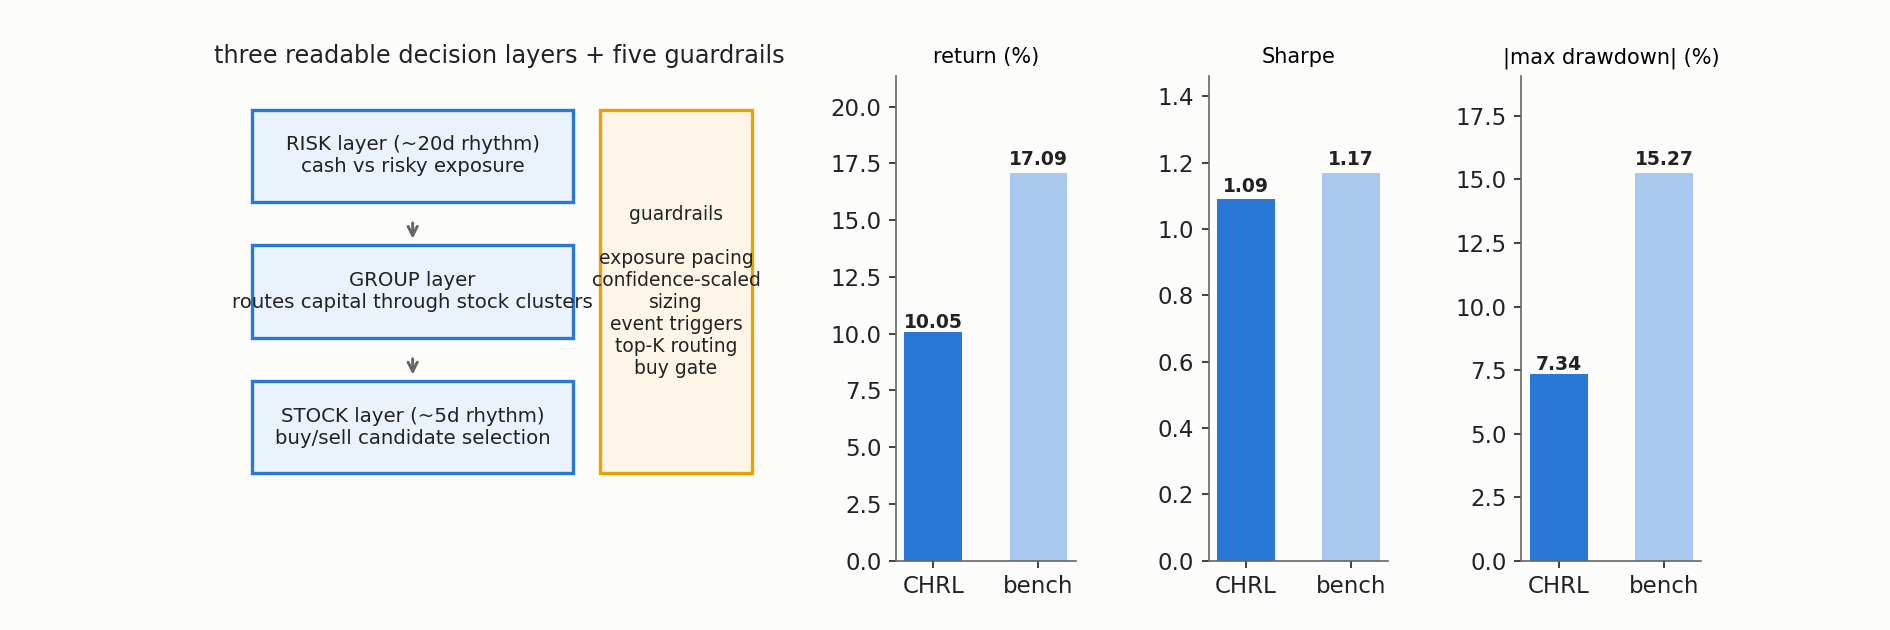
\includegraphics[width=\linewidth]{figures/fig_chrl.png}
  \caption{CHRL. Left: the three-layer decision factorization and its five guardrails --- each
  stage emits a loggable, auditable signal on its own rhythm. Right: four-fold walk-forward
  validation against the $100\%$-risky equal-weight benchmark: $58.8\%$ of the return,
  $93.2\%$ of the Sharpe, $52\%$ less drawdown.}
  \label{fig:chrl}
\end{figure}

So the layers are transparent, the guardrails are readable, and the trader is competent. The
question this paper turns on is what happens when you ask the next question: \emph{what is the
policy thinking between the layers?}

\section{Reading the black box: the Interpretable-CHRL program}
\label{sec:interp}

Before replacing an architecture on interpretability grounds, one owes it the strongest
post-hoc reading one can produce. We therefore ran a dedicated program (Interpretable-CHRL)
over the \emph{frozen} trained policy --- no reward change, no re-optimization, no re-fit ---
asking one question with increasing precision: \emph{which latent structures are actionable
under controlled intervention?}

\subsection{The staged pipeline}
\label{sec:stages}

The program proceeds in stages over a frozen rollout (Figure~\ref{fig:interp}, left): log the
hidden states and action chunks; \emph{discover} primitives by unsupervised clustering; label
them behaviorally from the trading logs; attach outcome diagnostics; and only then intervene.
The discovery stage yields a compact vocabulary with healthy statistics: a $K{=}8$ K-means
codebook with utilization $1.000$ (every primitive is used), perplexity $6.91$ (usage is
spread, not collapsed), median run length $18$ trading days (primitives are \emph{episodes},
not jitter), and cross-fold normalized mutual information $0.634$ (the vocabulary largely
replicates on held-out folds). The interventions themselves are one edit deep: take the
policy's own hidden state $h_t$, push it along an interpretable direction $d$ with strength
$\alpha$, and pass the edited state through the \emph{original} frozen action head,
\begin{equation}
\tilde h_t \;=\; h_t + \alpha\, d, \qquad
\tilde a_t \;\sim\; \pi_\theta(\,\cdot \mid \tilde h_t\,),
\label{eq:intervene}
\end{equation}
so any behavioral change is attributable to the edit alone. Five intervention families are
tested, each phrased as a falsifiable question:
\begin{center}\small
\begin{tabular}{lp{10.2cm}}
\toprule
type & question \\
\midrule
suppression & does damping a locally harmful primitive improve the counterfactual rollout? \\
promotion & does amplifying a locally beneficial primitive improve it? \\
best-context map & does the best primitive depend on market regime (train-only target)? \\
replacement & does substituting a context-appropriate primitive for a weak one improve it? \\
repair & do a few targeted, context-conditional edits beat matched random alternatives? \\
\bottomrule
\end{tabular}
\end{center}

\subsection{What post-hoc buys --- under controls}
\label{sec:interpresults}

The central methodological lesson arrived immediately: on this substrate, a \emph{random-target
joint} edit (hidden state $+$ hidden action) also ``improves'' the frozen 2022--23 rollout
($+0.552$\,pp) --- gentle noise perturbs a locally suboptimal policy off its habits. Every claim below is therefore
\emph{control-adjusted}: the reported value is the targeted edit's delta minus its matched-random
twin's (Figure~\ref{fig:interp}, right). Under that discipline, three results survive. First,
hidden states are control surfaces: promoting a specific primitive yields $+0.540$\,pp raw but
$+0.263$\,pp control-adjusted ($+0.049$ Sharpe); replacing a weak primitive with its
context-best alternative yields $+0.421$\,pp raw, $+0.302$\,pp adjusted. Second, hidden
\emph{actions} are too: a learned adapter on the action pathway gives $+0.377$\,pp raw,
$+0.265$\,pp adjusted. Third, the effects are specific: adding targeted repairs of two diagnosed primitives to the
joint promotion baseline reaches $+0.508$\,pp where the matched random-repair control reaches
only $+0.316$\,pp ($+0.192$\,pp of specificity). Post-hoc analysis is not nothing; we state this against our own
thesis: it found real, modular, editable structure inside a policy that was never built to have
any.

\begin{figure}[t]
  \centering
  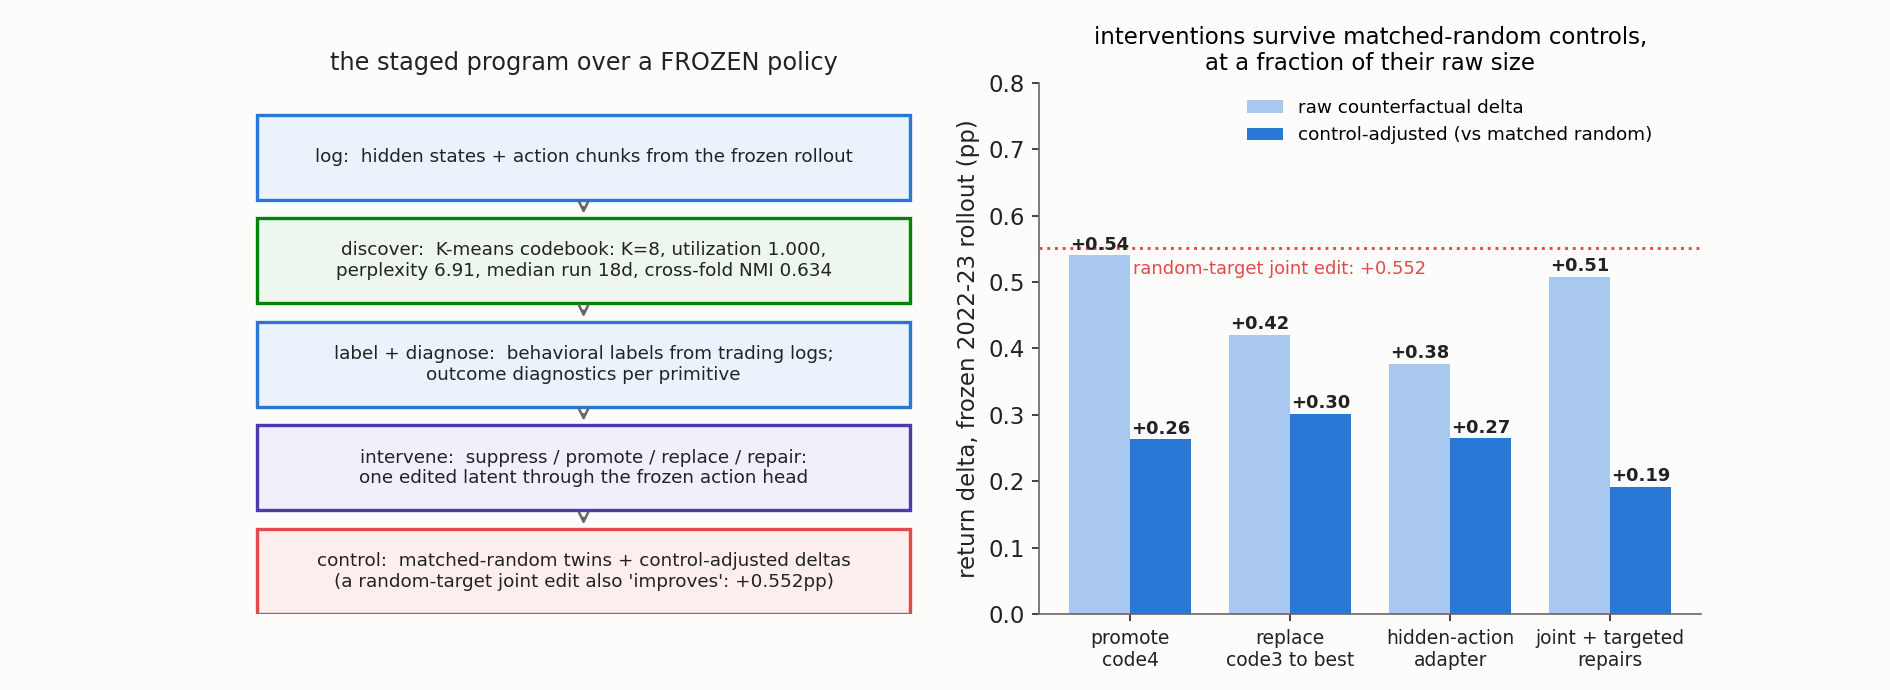
\includegraphics[width=\linewidth]{figures/fig_interp.png}
  \caption{The Interpretable-CHRL program. Left: the staged pipeline over the frozen policy ---
  log, discover ($K{=}8$ codebook; utilization $1.000$; perplexity $6.91$; median run $18$d;
  cross-fold NMI $0.634$), label, diagnose, intervene (Eq.~\ref{eq:intervene}), control. Right:
  the flagship counterfactuals on the frozen 2022--23 rollout, raw vs control-adjusted; the
  dotted line is the random-target joint edit ($+0.552$\,pp) that makes control adjustment
  mandatory.}
  \label{fig:interp}
\end{figure}

\subsection{Where post-hoc stops}
\label{sec:wall}

The same program measures its own ceiling, and every question we most cared about hit the same
wall. \emph{Memory}: the policy's state is smeared through the network, so no bound exists on
what a hidden-state edit can touch --- the matched-random result above is exactly the symptom
(noise moves behavior about as much as intention; only the \emph{difference} is knowledge).
\emph{Commands}: the control surface is ${\sim}214$ engineering knobs, none of which is a
semantic command; steering means forcing the latent toward a post-hoc K-means centroid and
checking that behavior moves \emph{consistently} --- a correlation, not an intervention.
\emph{Story}: when we scored the deployed agent's own stance log on the simulatability metric of
\S\ref{sec:metrics}, a $K{\le}9$ named story reproduced only $0.244$ of its behavior --- the
latent is genuinely incompressible at a human-story budget. And \emph{scope}: all counterfactual
evidence lives on one frozen, stress-heavy window (2022--23), because the frozen-policy
discipline that makes the measurements clean also chains them to a fixed rollout. Transparent
layers, opaque core. The program's own stated next step --- ``turn the primitive-level signal into a cleaner
training-time objective or policy-improvement loop'' --- is the bridge this paper crosses: instead of discovering
primitives after training, \emph{build the agent out of named parts}.

\section{CRYSTAL-1: legible by construction}
\label{sec:crystal}

CRYSTAL-1 rebuilds the core around three commitments, each a direct answer to a measured
failure of \S\ref{sec:wall} (Figure~\ref{fig:arch}).

\paragraph{1. Memory is a named posterior.} The agent's only recurrent state is a belief over
$K$ market regimes --- a point on the simplex $\Delta^{K-1}$ --- in the POMDP sense of a belief
state \citep{kaelbling1998}, over Hamilton-style regimes \citep{hamilton1989}. For the $K{=}2$
US machinery, with regime densities $f_z(r) = \mathcal{N}(r;\mu_z,\sigma_z^2)$,
$z\in\{\text{bull},\text{bear}\}$, and a sticky transition prior $\pi_{zz'}$, the belief is the
explicit Hamilton filter
\begin{align}
b_t \;=\; \Prob(z_t = \text{bear}\mid \mathcal{F}_t)
\;&=\; \frac{f_{\text{bear}}(r_t)\,\tilde b_t}
{f_{\text{bear}}(r_t)\,\tilde b_t + f_{\text{bull}}(r_t)\,(1-\tilde b_t)},
\label{eq:belief}\\
\tilde b_t \;&=\; \pi_{BB}\, b_{t-1} + \pi_{GB}\,(1-b_{t-1}),\nonumber
\end{align}
where $\mathcal{F}_t$ is the information available at $t$ (\S\ref{sec:data}). \emph{Named} is
load-bearing: because the coordinate has a meaning, a write to the belief is a sentence
(``believe bear at $0.8$''), and because $b_t$ is the sole memory channel, the blast radius of
any memory intervention is bounded by construction --- the property Eq.~\ref{eq:intervene}
could test for but never guarantee.

\paragraph{2. The policy head is the story.} The decision layer is a small tree over
$[\,b_t,\ \text{inventory},\ \text{time}\,]$. In the soft form \citep{frosst2017} each inner
node $i$ routes by a sigmoid gate and each leaf $\ell$ holds a distribution over actions:
\begin{align}
p_i(x) &= \sigma\!\big(\beta(w_i^{\top}x + c_i)\big), \qquad
P^{\ell}(x) = \prod_{i \in \text{path}(\ell)} p_i(x)^{\ind[\ell \swarrow i]}
\big(1-p_i(x)\big)^{\ind[i \searrow \ell]},
\label{eq:tree}\\
\pi(a\mid x) &= \sum_{\ell} P^{\ell}(x)\, Q^{\ell}_a ,\nonumber
\end{align}
with the inverse temperature $\beta$ annealed so the trained tree is effectively hard. The
constraint is that the tree \emph{is} the policy --- there is no residual network for behavior
to hide in --- and it must pay no performance tax (\S\ref{sec:compare}). At the limit the
readable rule degenerates to a sentence; the certified US rule of \S\ref{sec:cert} is literally
\begin{equation}
e_t \;=\; \begin{cases} 0.74, & b_t > 0.66\\[2pt] 1.00, & \text{otherwise,}\end{cases}
\label{eq:rule}
\end{equation}
where $e_t$ is the equity exposure.

\paragraph{3. Commands are few, named, and governed.} The ${\sim}214$-knob surface collapses to
\textbf{five agent-facing levers}:
\begin{center}\small
\texttt{SET\_BELIEF} \,\textperiodcentered\, \texttt{EXPOSURE\_MODE} \,\textperiodcentered\,
\texttt{GROUP\_CONCENTRATION\_CAP} \,\textperiodcentered\,
\texttt{ABSTAIN\_FLOOR} \,\textperiodcentered\, \texttt{DRAWDOWN\_BUDGET}
\end{center}
(the concentration cap is \emph{hard}, fixing the predecessor's soft-cap failure). Everything
else is engineering-fenced. A write is the \emph{do}-operator of \citet{pearl2009} made
concrete: $\texttt{SET\_BELIEF}(b^{*}, w)$ realizes
\begin{equation}
b_t \;\leftarrow\; (1-w)\, b_t + w\, b^{*}, \qquad w \in [0,1],
\label{eq:write}
\end{equation}
and a \emph{dose} nudge of $\delta$ nats acts in log-odds,
$\operatorname{logit}(b_t) \leftarrow \operatorname{logit}(b_t) + \delta$. Writes must pass a
non-inferiority bar on the certified objective before they are allowed to persist
(\S\ref{sec:compare}).

\begin{figure}[t]
  \centering
  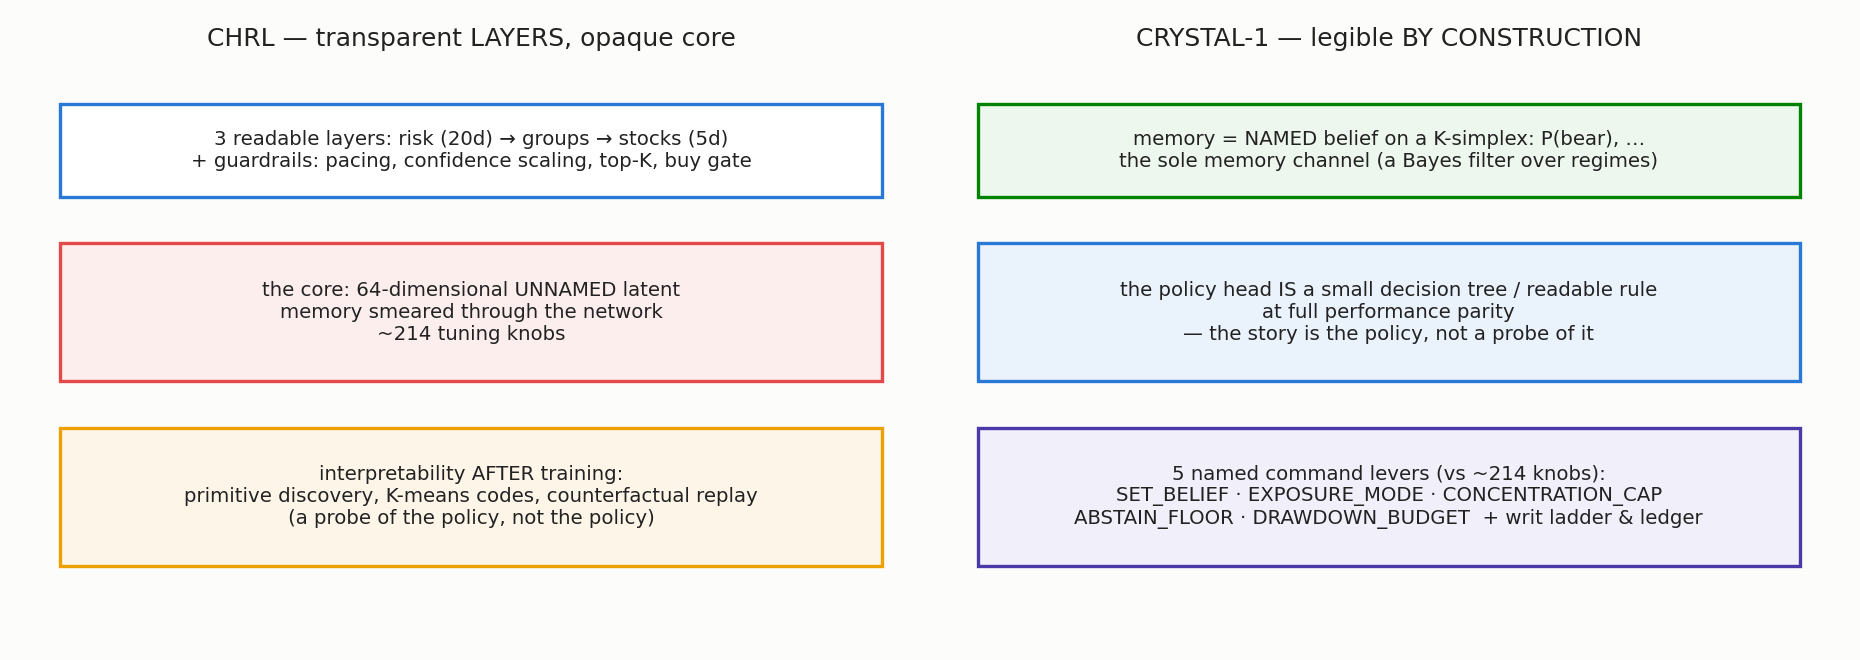
\includegraphics[width=\linewidth]{figures/fig_architectures.png}
  \caption{The journey in one picture. CHRL factors decisions into readable layers but keeps an
  unnamed 64-d latent core with ${\sim}214$ knobs, explained only after training
  (\S\ref{sec:interp}). CRYSTAL-1 makes the explanation the mechanism: a named belief as the
  sole memory channel, a readable rule as the policy itself, and five named command levers.}
  \label{fig:arch}
\end{figure}

\section{Data and evaluation}
\label{sec:data}

All quantitative claims are computed on real market data under point-in-time (PIT) discipline.
The universe is daily total-return series for six liquid US-listed assets plus cash --- SPY
(US large-cap equities), EFA (developed ex-US), IEF and TLT (7--10y and 20y+ Treasuries), TIP
(inflation-linked), GLD (gold), with the 13-week T-bill rate as the cash leg --- split- and
dividend-adjusted closes converted to total-return relatives, the cash leg accruing
$r^f_t = y_t/252$. The exposure-rule experiments (\S\ref{sec:compare}) additionally use the
lab's Dow-30 daily panel (2000--2026). Every panel enters through a signed data gate (file
hash, source URL, vintage recorded before any experiment may read it) and is ground-truthed
against an independent source --- a discipline bought by experience: a Chinese panel once
passed every internal consistency check while carrying a mixed clock (close and volume lagged a
day against high and low); only external ground-truthing caught it, and every result computed
on that panel was voided. A decision issued at $t$ may use only
$\mathcal{F}_t = \sigma(\{x_s : s\le t\})$, with publication lags respected; evaluation stands
at historical origins and is scored on realized continuations, never re-fit on them.

Two evaluation formulas recur. For a daily excess-return sequence $x_t$ and wealth path $W_t$:
\begin{equation}
\text{Sharpe} = \frac{\sqrt{252}\,\overline{x}}{\hat\sigma(x)}, \qquad
\text{max drawdown} = \min_{t}\Big(\frac{W_t}{\max_{s\le t} W_s} - 1\Big).
\label{eq:mdd}
\end{equation}
The goal-planning machinery that CRYSTAL-1 serves in production --- scenario kernels by
stationary bootstrap \citep{politis1994}, dynamic programming on the funding ratio
\citep{das2020goals,browne1999}, and the promise backtests --- is specified and evaluated in
the companion paper (\emph{Hello Crystal}); here we use only its policy \emph{tables}, which
are the objects the simulatability metric reads.

\section{CrystalScore: measuring ``legible'' so it can lose}
\label{sec:metrics}

A legibility claim that cannot lose is marketing. We score every architecture with
\begin{equation}
\textsc{CrystalScore} \;=\; F \times S \times S\!t,
\label{eq:cs}
\end{equation}
at a fixed parsimony budget $K \le 9$ (at most nine named rules/leaves), with each axis
operationalized so that it \emph{could have} come out low
\citep{doshivelez2017,jacovi2020,lipton2018}:
\begin{align}
F \text{ (faithfulness)} &= \E\Big[\ind\big[\pi\big(b \leftarrow \operatorname{do}(b^{*})\big)
= \pi^{*}(b^{*})\big]\Big],
\label{eq:faith}\\[3pt]
S \text{ (simulatability)} &= \operatorname{acc}\big(\text{story}_{K},\, \pi\big)
\ \ \text{s.t.}\ \ \big|\mathcal{R}(\text{story}_K) - \mathcal{R}(\pi)\big| \le \varepsilon,
\label{eq:simul}\\[3pt]
S\!t \text{ (stability)} &= \frac{1}{n}\sum_{i=1}^{n}
\ind\big[\text{mechanism replicates on seed } i\big].
\label{eq:stab}
\end{align}
Faithfulness (Eq.~\ref{eq:faith}): \emph{do}-writes must land, judged against a reference
optimum, not against the policy's own habits. Simulatability (Eq.~\ref{eq:simul}): a $K$-rule
story must match the policy \emph{at performance parity} $\mathcal{R}$ --- a story that
reproduces a lobotomized policy is cheating. Stability (Eq.~\ref{eq:stab}): the mechanism must
replicate across independent training seeds. The non-saturating companion is the \textbf{MDL
deficit} \citep{rissanen1978},
\begin{equation}
\Delta_{\text{MDL}} \;=\; \operatorname{Acc}(\pi) - \operatorname{Acc}(\text{story}_{K}),
\label{eq:mdl}
\end{equation}
the accuracy lost by forcing the explanation to be short; $0$ means a short story loses
nothing.

\paragraph{A measurement correction, reported as a finding.} Faithfulness probes can silently
lie. Our original probe applied fixed-size belief writes ($+0.2/+0.4$) and checked whether the
action followed. On threshold policies whose belief input saturates, such writes never cross
the decision boundary --- so a policy that \emph{is} the rule by construction (a behavior-cloned
distillation with accuracy $0.97$) read $F{=}0.00$. The repaired protocol uses matched-state
\emph{contrast writes} ($b{=}0.2$ vs $b{=}0.8$, spanning both certified thresholds). Under the
corrected probe, cold-trained RL heads remain unfaithful under both probes ($F$ strict $0.00$,
contrast $0.00$), while teacher-warm-started heads score contrast-write $F = 0.77$--$0.83$ where
the strict probe read $0.03$ (\S\ref{sec:compare}). The lesson generalizes: \emph{an
interpretability metric is an instrument, and instruments need calibration surfaces} --- this
one was caught on a designed environment where ground truth was known by construction
(\S\ref{sec:polygon}).

\paragraph{Real-data values.} On its own deployed-panel stance log, the CHRL-line agent scores
$F{=}1.00$ (latent steering does move behavior --- faithfulness alone cannot distinguish the
designs), $S{=}0.244$ (\S\ref{sec:wall}), $S\!t{=}0.619$:
$\textsc{CrystalScore}{=}0.151$. CRYSTAL-1's axes on the real US machinery: $S{=}0.92$ (an
8-leaf tree reproduces the goal-planner champion's policy table at parity); $S\!t{=}1.00$ (the
certified rule's behavior replicates on 10/10 training seeds); $F{=}1.00$ (writing the bear
belief past the threshold changes exposure exactly as named); $\Delta_{\text{MDL}}{=}0.0$:
$\textsc{CrystalScore}{=}0.92$ (Figure~\ref{fig:crystalscore}). The entire $6\times$ gap is
Simulatability --- exactly what ``born legible'' buys. Alpha does not enter the score.

\begin{figure}[t]
  \centering
  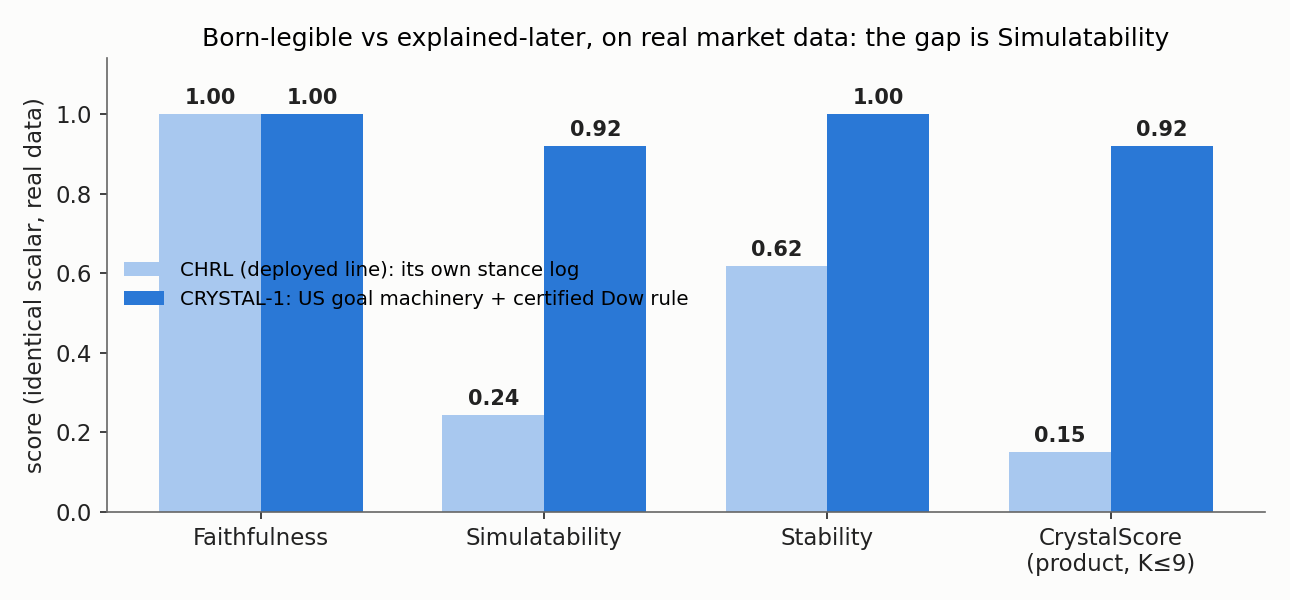
\includegraphics[width=.9\linewidth]{figures/fig_crystalscore.png}
  \caption{The identical scalar on both architectures, real data only: the CHRL line is scored
  on its own deployed-panel stance log; CRYSTAL-1 on the US goal machinery (tree-vs-champion
  simulatability) and the certified Dow rule (10-seed stability, write fidelity). Faithfulness
  is $1.0$ for both --- steering works on a black box too; the discriminating axis is whether a
  $K{\le}9$ named story can reproduce behavior at parity.}
  \label{fig:crystalscore}
\end{figure}

\section{The comparison: influence, certification, and the final table}
\label{sec:compare}

A legible agent is only useful if you can \emph{change} it on purpose. We exercised four
families of influence on CRYSTAL-1's PPO reward-dial heads --- a research prototype, not the
champion --- on the real US daily panel (train 2010--18, held-out evaluation after), each with
a control battery so we report what the levers actually do, not what they appear to
(Figure~\ref{fig:levers}).

\paragraph{R --- reward shaping.} The risk-targeted reward
\begin{equation}
r_t \;=\; e_t\, x_t \;-\; \lambda_{R}\,\max\big(0,\ \text{DD}_t - D^{*}\big)
\label{eq:reward}
\end{equation}
($e_t$ exposure, $x_t$ the asset return, $\text{DD}_t$ running drawdown, $D^{*}$ the budget)
moves the exposure dial, but the penalty \emph{alone does not enforce the budget}: only the
$5\%$ head holds its budget ($-4.81\%$ held-out max drawdown, by parking in cash) while the
$8\%$ and $12\%$ heads breach theirs ($-15.9\%$). A drawdown-matched twin shows $z = 0.00$
timing skill: reward shaping buys \emph{risk placement}, not timing. Enforcing the budget
requires a separate constrained objective (a Lagrangian head drives the breach down at a
$15$--$37$\,pp goal-probability cost) --- one more reason the transparent planner, which
respects capacity by a hard pre-filter, stays champion.

\paragraph{T --- teachers.} Trained cold, the heads' argmax behavior looked sensible while the
underlying preferences were nearly flat --- an effectively untrained network masked by
deterministic evaluation (mean max action-probability $0.21 \approx 1/5$). The cure is behavior
cloning from the certified rule (Eq.~\ref{eq:rule}),
$L_{\text{BC}}(\theta) = -\E_{(s,a^{*})}[\log \pi_\theta(a^{*}\mid s)]$, $87\%$ agreement, used
as a warm start \citep{ross2011dagger,rusu2016distillation}: mean max action-probability
$0.21 \to 0.73$, the belief becomes load-bearing, and the corrected contrast-write probe
(\S\ref{sec:metrics}) shows the teacher installs the rule's \emph{causal} belief$\to$action
structure ($F = 0.77$--$0.83$), which PPO fine-tuning does not erode on this substrate. Cold
discovery still fails; teaching works. (Leakage note: this teacher was \emph{selected} on the
2022--23 hold, so its hold read is contaminated; the leak-free teacher in the pipeline is the
planner champion, and a fresh read is pre-registered for 2027.)

\paragraph{I --- interventions, under controls.} The honest result overturns a first-pass
claim. On the cold reward-dial heads, belief writes and per-primitive promotions \emph{appear}
to steer behavior --- but a matched-random leaf moves behavior exactly as much as the targeted
one (the placebo fails), and belief-write fidelity is $3\%$: the apparent steering was a
near-uniform-head artifact, precisely the failure mode \S\ref{sec:interpresults}'s controls
exist to catch. What survives is the refusal machinery: the certification gate correctly
refuses a $+1$-nat promotion that fails the non-inferiority test
\begin{equation}
\text{accept the write} \iff \widehat{J}_{\text{post}} \ \ge\ \widehat{J}_{\text{pre}} -
\delta_{\text{NI}},
\label{eq:ni}
\end{equation}
and likewise rejects on the hold a reward ``winner'' selected on development ($z=1.34 < 2.15$).

\paragraph{A --- architecture.} Tree depth is a legibility dial set before training: depth-2
yields a 4-leaf policy, depth-3 the 8-leaf one. Scoring the prototype head itself: perfectly
simulatable ($S{=}1.0$; a 4-leaf story distills the 8-leaf head exactly) and stable
($S\!t{=}1.0$, 3 seeds) but --- when cold --- not faithful ($F{=}0.03$;
$\textsc{CrystalScore}{=}0.03$): a legible, stable \emph{dial}, not a command surface. The
faithful command surface is either taught (lever T) or built (the champion's rule, $F{=}1.0$).

\begin{figure}[t]
  \centering
  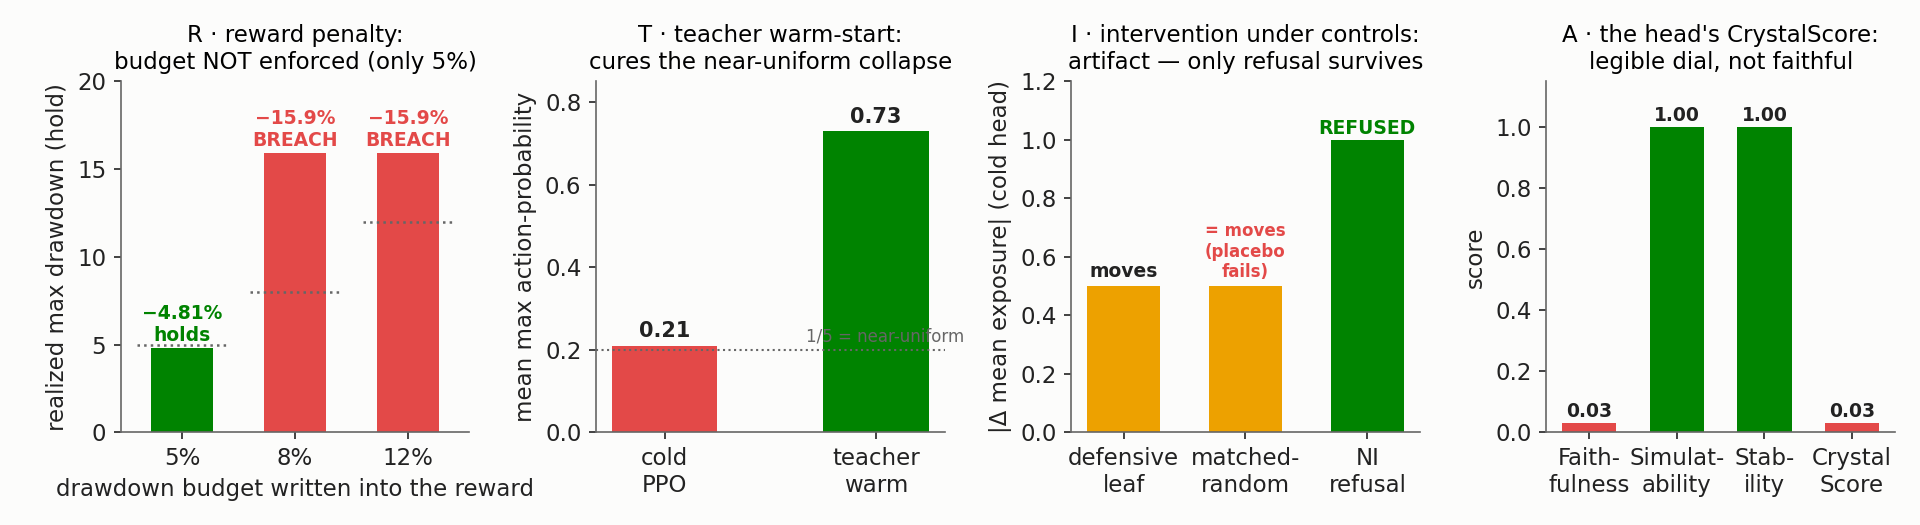
\includegraphics[width=\linewidth]{figures/fig_levers.png}
  \caption{The four influence levers on the real daily panel, under controls. R: the reward
  penalty holds only the $5\%$ budget --- the penalty does not enforce the budget. T: the
  teacher warm-start cures the cold near-uniform collapse ($0.21\to0.73$; corrected
  contrast-write $F=0.77$--$0.83$). I: a matched-random leaf moves the cold head as much as the
  targeted one --- only the non-inferiority \emph{refusal} (Eq.~\ref{eq:ni}) survives. A: the
  cold head is a legible, stable dial ($S{=}1.0$, $S\!t{=}1.0$, $F{=}0.03$), not a faithful
  command surface.}
  \label{fig:levers}
\end{figure}

\subsection{A certified readable rule on untouched data}
\label{sec:cert}

The self-improvement loop's frozen certification gate (specified in the companion paper) has
certified exactly one real-data policy to date --- and it is a sentence (Eq.~\ref{eq:rule}). It
entered with 7 accepts and \textbf{0} placebo accepts, and held one-shot on 629 untouched
trading days: Sharpe $1.46$ vs $1.39$ buy-and-hold, max drawdown $-12.9\%$ vs $-15.5\%$,
risk-adjusted improvement $z = +2.06$. The claim is a \emph{risk} claim (same return,
meaningfully less pain), certified as such; a written return-improvement rule was separately
tested and closed ($-8.8\%$). The rule's machinery was then audited on the real panel: naming
faithfulness $1.0$ (the state called ``bear'' is the state in which de-risking is optimal under
the world model); 10-seed behavioral stability $1.0$; rule re-discovery from scratch $3/3$;
belief MDL deficit $0.0$. These are the CRYSTAL-1 entries of Figure~\ref{fig:crystalscore} and
Table~\ref{tab:final}.

\begin{table}[h]
\centering\small
\begin{tabular}{p{3.4cm}p{5.2cm}p{5.2cm}}
\toprule
 & \textbf{CHRL} & \textbf{CRYSTAL-1} \\
\midrule
Memory & 64-d unnamed latent, smeared; blast radius unboundable & named posterior $b_t$
(Eq.~\ref{eq:belief}); the sole memory channel \\
Policy legibility & post-hoc codes over a continuous latent; story acc.\ $0.244$ & the policy
\emph{is} a table/rule; 8-leaf story acc.\ $0.92$ at parity \\
Steering primitive & force the latent toward a K-means centroid (correlation; matched-random
controls mandatory) & named \emph{do}-write (Eq.~\ref{eq:write}), fidelity $1.0$ \\
Refusals & OOD gate shrinks or zeroes steps & the NI bar (Eq.~\ref{eq:ni}) refused a $+1$-nat
promotion \\
Control surface & ${\sim}214$ knobs & 5 named levers \\
Seed stability & $0.619$ & $1.00$ (10 seeds) \\
\textsc{CrystalScore} (Eq.~\ref{eq:cs}) & $\mathbf{0.151}$ & $\mathbf{0.92}$ \\
Flagship real-data result & walk-forward: Sharpe $1.09$, maxDD $-7.34\%$; control-adjusted
targeted edits $+0.19$--$0.30$\,pp & certified rule, 629 untouched days: Sharpe $1.46$ vs
$1.39$, maxDD $-12.9\%$ vs $-15.5\%$ \\
Deployment status & deployed: live firewall, operating history & goal machinery live on the US
universe (paper track); client certification still \emph{refused}, with dated unlocks \\
\bottomrule
\end{tabular}
\caption{The final comparison, real data only. The honest split: CHRL remains the
longer-operating deployed system, and its post-hoc program found real editable structure;
CRYSTAL-1 wins every legibility and control axis and carries its own real-data results, while
its client-facing certification correctly refuses until the pre-registered reads mature.}
\label{tab:final}
\end{table}

\section{The designed-market experiment: can a market reward only a clean mind?}
\label{sec:polygon}

Real markets have very noisy logic: the regime is largely priced, so the honest value of even a
perfect regime belief can be zero --- and a null result on real data cannot distinguish ``the
instrument is broken'' from ``there was nothing to detect.'' This motivates one deliberately
synthetic experiment: \emph{can one build a market that rewards only a ``clean'' mind --- an
environment where the belief information carries value by construction, so that command-surface
machinery can be calibrated at all?}

We built such an environment (a regime market whose returns are generated from latent states
the belief can, in principle, track) and used it strictly as \textbf{instrument calibration}.
On it: belief writes were \emph{proved} causal against an exogenous belief-MDP optimum
(agreement $0.80$/$0.835$ for the two heads); a likelihood-based \emph{lie detector} separates
sharp-but-wrong commands from uncertain-but-right ones (excess predictive NLL $0.43$ vs
${\approx}0$; detection $0.71$ at $5\%$ false alarms) while the na\"ive entropy gate points
\emph{backwards} (it trusts the confident lie); a 216-cell factorial showed command composition
is non-additive with \emph{sign-flipping} cross-terms (median $|\varepsilon| = 2.66$) --- which
is why the write surface is governed by a calibrated ledger, a co-activation cap, a kNN
manifold governor ($24/24$ engineered off-manifold corners flagged at $1.2\%$ held-out FPR) and
a writ ladder with a first false-accept estimate ($0/48$; $\lesssim 6\%$ by the rule of three).
On a \emph{hard} designed substrate the gate also certified a genuine
return$\leftrightarrow$legibility \emph{tension} --- legibility is not free everywhere, and
anyone claiming otherwise is measuring easy tasks. It was also this environment that exposed
the faithfulness-probe blindness of \S\ref{sec:metrics}.

The bridge back to reality is an explicit \textbf{value-of-information gate}
(Figure~\ref{fig:polygon}): the designed market shows VoI $= 5.92$ ($+282\%$ of a belief-blind
baseline) and the gate \emph{opens}; on a real book the measured VoI is $0$ and the gate
\emph{closes} --- so nothing calibrated on the designed market is allowed to generate a
real-market claim, and no designed-market number appears in \S\ref{sec:compare}.

\begin{figure}[t]
  \centering
  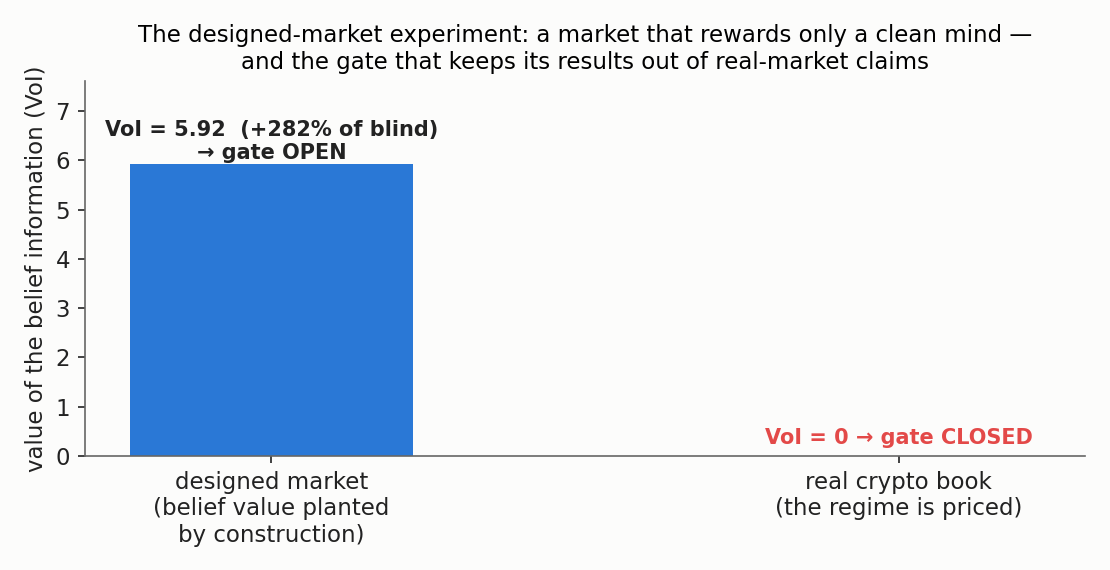
\includegraphics[width=.72\linewidth]{figures/fig_polygon.png}
  \caption{The designed-market experiment and its fence. Left: the environment built to reward
  a clean mind --- belief information worth $+282\%$ of blind by construction, so command
  machinery (causal writes, the lie detector, composition governance, probe calibration) can be
  calibrated. Right: the same measurement on a real book returns zero, and the gate closes.}
  \label{fig:polygon}
\end{figure}

\section{What did not work, and what bounds the claims}
\label{sec:nulls}

A paper about honest machinery should list its own falsifications; each cost us a believed
hypothesis, and the machinery that killed them is part of the contribution. (i) \textbf{Raw
counterfactual lifts were inflated ${\sim}2\times$}: a random-target joint edit
``improves'' the frozen rollout by $+0.552$\,pp (\S\ref{sec:interpresults}) --- without matched
controls, every post-hoc intervention result in \S\ref{sec:interp} would have been
overstated. (ii) \textbf{The strict faithfulness probe read $F{=}0.00$ on a policy that was
the rule by construction} (\S\ref{sec:metrics}) --- an uncalibrated interpretability metric
lied in the pessimistic direction. (iii) \textbf{Cold RL heads are not command surfaces}: the
placebo fails, write fidelity is $3\%$; only teaching or building installs causal structure
(\S\ref{sec:compare}). (iv) \textbf{A written return-improvement rule closed} ($-8.8\%$): the
certified claim is risk-shaped, not alpha-shaped. (v) \textbf{A PPO challenger loses to the
readable planner table} on the same action space (regret $6.6$\,pp) --- reported because the
field's default is the opposite claim. (vi) \textbf{Legibility is provably not free} on a hard
designed substrate (the certified tension of \S\ref{sec:polygon}). (vii) \textbf{Post-hoc
interpretability was not worthless}: it found the load-bearing concepts (motifs, codes,
counterfactual replay) that CRYSTAL-1 promoted from probes into architecture --- the right
summary is that building them in made the story ${\sim}4\times$ more compressible ($0.244 \to
0.92$ at the same budget).

\section{Related work}
\label{sec:related}

Interpretability-by-construction vs post-hoc explanation \citep{rudin2019,lipton2018}; rigor
and evaluation of interpretability \citep{doshivelez2017,hoffman2018}; faithfulness as a
criterion \citep{jacovi2020}. CRYSTAL-1's named belief is a concept-bottleneck design in the
sense of \citet{koh2020} --- the belief is a supervised, human-named intermediate through which
all memory must pass --- with the difference that our bottleneck is also the \emph{write}
surface, so faithfulness is tested by intervention (Eq.~\ref{eq:faith}), not only by probe
accuracy; and where circuit-style analysis \citep{olah2020} reverse-engineers named structure
\emph{out of} trained networks, CrystalRL builds the named structure \emph{in} and reserves
reverse-engineering for the audit. Belief-state control \citep{kaelbling1998} and regime models
\citep{hamilton1989} supply the named memory; soft trees \citep{frosst2017} the legible head;
MDL \citep{rissanen1978} the non-saturating ruler; interventional causality \citep{pearl2009}
the faithfulness protocol. Discretized latent-action behavior generation \citep{lee2024vqbet}
pursues the complementary direction --- learned discrete codes for \emph{expressiveness} ---
where CrystalRL fixes the codes to \emph{named} coordinates for legibility. Hierarchical RL as
partial legibility \citep{sutton1999options,bacon2017option}; PPO and constrained variants
\citep{schulman2017ppo,achiam2017}; goal-conditioned value functions \citep{schaul2015};
imitation-then-optimize \citep{ross2011dagger,rusu2016distillation}; reward shaping
\citep{ng1999shaping}; goal-based planning \citep{das2020goals,browne1999}; the stationary
bootstrap \citep{politis1994}. The self-improvement layer --- LLM proposers over verified
evaluators \citep{romera2024funsearch,novikov2025alphaevolve,ma2023eureka,wang2023voyager} and
the statistics of adaptive search over noisy financial evaluators \citep{baileylopez2014dsr}
--- is treated in the companion paper (\emph{Hello Crystal}); this paper builds the object
those loops are allowed to modify.

\section{Conclusions: what the journey establishes about interpretable RL}
\label{sec:conclusions}

Five findings travel beyond this system.

\textbf{1. The discriminating axis is simulatability, not faithfulness.} Steering ``works'' on
a black box too ($F{=}1.0$ for both architectures); what born-legible buys is that a $K{\le}9$
named story reproduces behavior at performance parity ($0.244 \to 0.92$). Evaluations of
interpretable RL that report only intervention success are measuring the wrong axis.

\textbf{2. Post-hoc analysis finds structure but cannot bound it.} The strongest post-hoc
program we could run found a real, complete, editable primitive vocabulary --- and still could
not bound the blast radius of an edit, name a command, or compress the policy into a story.
The two families are not rivals: post-hoc discovery told us \emph{which} concepts to build into
the successor.

\textbf{3. Controls and calibration are not optional.} A random-target edit improves the
rollout ($+0.552$\,pp); a placebo leaf moves a cold head as much as the targeted one; a strict
faithfulness probe reads $0.00$ on a policy that is the rule by construction. Every
interpretability measurement in this paper that lacked a control or a calibration surface was
wrong on the first pass --- always in a direction favorable to a good story.

\textbf{4. Causal command structure is taught or built, never free.} Cold RL training produced
legible, stable \emph{dials} with near-zero faithfulness; behavior cloning from a certified
readable rule installed the causal belief$\to$action structure ($F = 0.77$--$0.83$) and PPO
fine-tuning did not erode it. If you need a command surface, put it there on purpose.

\textbf{5. Legibility is not free everywhere --- and where it is expensive is informative.} On
an easy substrate the readable rule pays no tax; on a hard designed substrate a certified
return$\leftrightarrow$legibility tension appears. Mapping \emph{where} the tension binds is a
better research question than asserting either side of it.

The forward-looking program is falsifiable by design; its flagship hypotheses: machine
simulatability predicts \emph{human} simulatability (kill: humans at chance while the machine
metric is at ceiling); a legibility scaling law --- optimal vocabulary size $K$ tracks substrate
behavioral complexity (kill: no relation across universes); interpretability \emph{drift} ---
naming faithfulness decays under a self-improvement loop unless re-certified (kill: $F$ stays
$1.0$ over 20+ accepted changes); motif conservation --- CHRL's discovered primitives re-emerge
as CRYSTAL-1 rule clauses (kill: no better-than-chance correspondence); dose-response of
\texttt{SET\_BELIEF} is monotone and saturating on certified substrates (kill: non-monotone
regions); the composition ledger's cross-terms appear on the real panel's visited manifold
(kill of the premise: on-manifold interactions are additive); and CrystalScore transfers to the
\emph{improver} --- the coding agent's stated rationales predict its measured effects (kill:
rationale--effect agreement at chance, itself a publishable confabulation result).

\section{Limitations}
\label{sec:limits}
(i) The scenario-based probabilities that the goal machinery quotes remain uncalibrated
research estimates; the calibration gates and their dated forward reads (2027-07-12; an
untouched multi-year fold maturing 2029) live in the companion paper. (ii) The real-data
CrystalScore's simulatability axis is measured on the planner champion and the certified rule
family --- not yet on every head. (iii) The command-surface \emph{proofs} (causal writes
against an exogenous optimum, the lie detector, composition governance) are designed-market
calibrations (\S\ref{sec:polygon}); their real-data analogues are open hypotheses. (iv) All
Interpretable-CHRL counterfactuals live on one frozen, stress-heavy window (2022--23) by
design. (v) The certified rule is one rule family on one substrate; hardening across
substrates, seeds and profiles is the program's first milestone. (vi) Execution economics
beyond $10$\,bp switching costs (taxes, spreads, gaps) are only partially bounded.

\section*{Acknowledgments and drafting discipline}
Prepared \emph{write-paper-first} \citep{eisner-paper-first}. Experiments were run and logged
under the repository's honesty contract --- every entry names its null, its seed, and its worst
caveat --- in the spirit of \citet{feynman1974}: \emph{``The first principle is that you must
not fool yourself --- and you are the easiest person to fool.''} LLM coding agents (Claude,
Codex) operated the experimental loops under the stated controls; the agents propose, the gates
dispose. The author thanks Joseph Lynch for discussions on the interpretability track.

\bibliographystyle{plainnat}
\bibliography{refs}

\end{document}
